\documentclass[11pt]{article}
\usepackage{tocloft}
\usepackage{graphicx}
\usepackage{calc}
\usepackage{amssymb}
\usepackage{color}
\usepackage{xcolor}
\usepackage{lscape}
\usepackage{array}
\usepackage[sc]{mathpazo}
\usepackage{url}
\usepackage[final]{pdfpages}
\usepackage{amsmath}
\usepackage{pdfpages}

%\linespread{1.05}
\oddsidemargin=0pt
\evensidemargin=0pt
\textwidth=7.5in
\topmargin=0pt
\headheight=0pt
\headsep=0pt
\textheight=10in
% EXPERIMENTAL
%\parindent=0pt
%\parskip=3pt
\setlength{\parindent}{0cm}
\newcommand\secfont{\fontfamily{cmss}\selectfont}%\textwidth 5.5truein
\newcommand\pifheading[1]{{\secfont\textbf{#1}:}}
%\oddsidemargin -0.40truein
%\textheight 8.0truein
%\topmargin -0.25truein
\def\lo{
\mathrel{\raise.3ex\hbox{$<$}\mkern-14mu\lower0.6ex\hbox{$\sim$}}
}
\def\hi{
\mathrel{\raise.3ex\hbox{$>$}\mkern-14mu\lower0.6ex\hbox{$\sim$}}
}

\textwidth = 6.6 in
\textheight = 9.1 in
\oddsidemargin = -0.05 in
\evensidemargin = +0.05 in
\topmargin = -.1 in
\headheight = 0.0 in
\headsep = 0.0 in
\parskip = 0.06in
\newcommand\registered{{\ooalign{\hfil\raise .00ex\hbox{\scriptsize R}\hfil\crcr\mathhexbox20D}}}

%% Define a new 'leo' style for the package that will use a smaller font.
\makeatletter
\def\url@leostyle{%
  \@ifundefined{selectfont}{\def\UrlFont{\sf}}{\def\UrlFont{\small\ttfamily}}}
\makeatother
%% Now actually use the newly defined style.
\urlstyle{leostyle}

%\pagestyle{empty}
%\includeonly{previous,proposal_references}
%\includeonly{proposal_references}
%\includeonly{previous}

% TOC

\pagenumbering{gobble}

\begin{document}
%%%%%%%%%%%%%%%%%%%%%%%%%%%%%%%%%%%%%%%%%%%%%%%%%%%%%%%%%%%%%%%%%%%%%
\begin{center}
\textbf{\Large
AST101: Our Corner of the Universe \\
\vspace*{0.1cm}
Lab 8: Spectroscopy (II)
}

\color{red} Note: Since we are printing labs for you this week, we {\bf may} ask you to turn your lab document in to us this week. This is the best lab of the year; enjoy it!
\end{center}


\vspace*{0.5cm}

{\Large Name:}\vspace*{0.5cm}\\\hrule
{\Large Lab section:}\vspace*{0.5cm}\\\hrule
{\Large Group Members:}\vspace*{0.5cm}\\\hrule
\vspace*{0.5cm}

%%%%%%%%%%%%%%%%%%%%%%%%%%%%%%%%%%%%%%%%%%%%%%%%%%%%%%%%%%%%%%%%%%%%%

\section{Objectives}
\begin{itemize}
	\item To determine the colors in an atom's emission/absorption spectrum based only on knowledge of its energy levels
	\item To gain experience determining chemical composition from emission spectra
\end{itemize}



\section{Identifying Sources}


There are various objects in the room that generate emission spectra. One of them is hydrogen, which doesn't match any of the examples
on your reference. The others are on the set of reference spectra that are included as the back page of this lab handout. 

{\color{red}Tear off that set of reference spectra; you will use it throughout today's lab. }

Your group should circle around to all of the tables and look at the different sources. Look at each source and label the position of 
the emission lines on the spectra as closely as you can. (Notice that the scale in your spectrometer is marked in both nanometers and eV/photon, but that the colors are likely in the opposite order of your reference. That's okay; you can plot this either way, and what matters is the wavelength/energy of each line. So, when you are looking at these, you might say something like ``Mercury's emission spectrum has a very bright green line at 546 nanometers.'') 

Draw the positions of the emission lines as precisely as you can, even if you don't need to do so in order
to identify the gas in question; you'll need a record of their energies and wavelengths for the second part of this lab.

It will probably be easiest if you measure where all the lines are first, and then try to figure out which
element is which. Remember, one of them is hydrogen, which isn't on your reference; in the next section, you'll calculate its emission spectrum from scratch.


\begin{minipage}{0.1\textwidth}
	\begin{center}
		\Large Source \\ A
	\end{center}
\end{minipage}
\begin{minipage}{0.7\textwidth}
	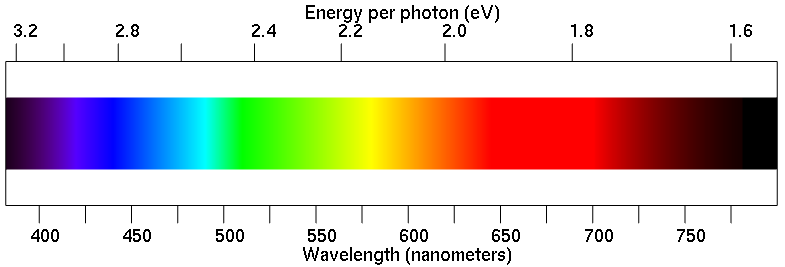
\includegraphics[width=\textwidth]{spectrum2.png}
\end{minipage}

\begin{minipage}{0.33\textwidth}
	What color \\does this appear?
\end{minipage}
\begin{minipage}{0.33\textwidth}
	What element is it?
\end{minipage}
\begin{minipage}{0.33\textwidth}
	What spectral lines did\\
	you use to identify it?
\end{minipage}

\vspace{1in}

\begin{minipage}{0.1\textwidth}
	\begin{center}
		\Large Source \\ B
	\end{center}
\end{minipage}
\begin{minipage}{0.7\textwidth}
	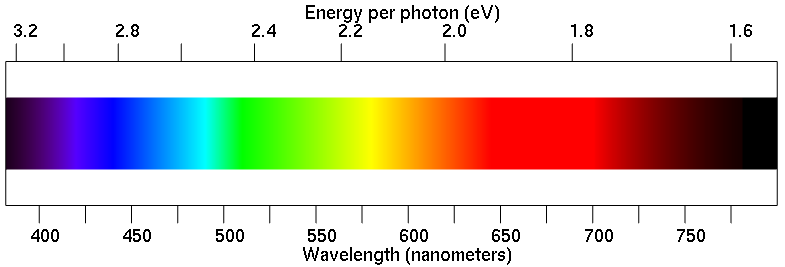
\includegraphics[width=\textwidth]{spectrum2.png}
\end{minipage}

\begin{minipage}{0.33\textwidth}
	What color \\does this appear?
\end{minipage}
\begin{minipage}{0.33\textwidth}
	What element is it?
\end{minipage}
\begin{minipage}{0.33\textwidth}
	What spectral lines did\\
	you use to identify it?
\end{minipage}

\vspace{1in}
\begin{minipage}{0.1\textwidth}
	\begin{center}
		\Large Source \\ C
	\end{center}
\end{minipage}
\begin{minipage}{0.7\textwidth}
	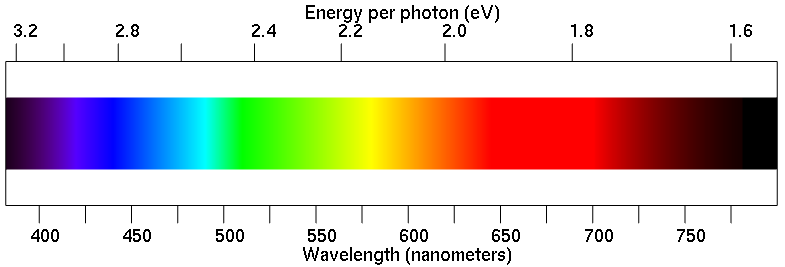
\includegraphics[width=\textwidth]{spectrum2.png}
\end{minipage}

\begin{minipage}{0.33\textwidth}
	What color \\does this appear?
\end{minipage}
\begin{minipage}{0.33\textwidth}
	What element is it?
\end{minipage}
\begin{minipage}{0.33\textwidth}
	What spectral lines did\\
	you use to identify it?
\end{minipage}

\vspace{1.2in}

\begin{minipage}{0.1\textwidth}
	\begin{center}
		\Large Source \\ D
	\end{center}
\end{minipage}
\begin{minipage}{0.7\textwidth}
	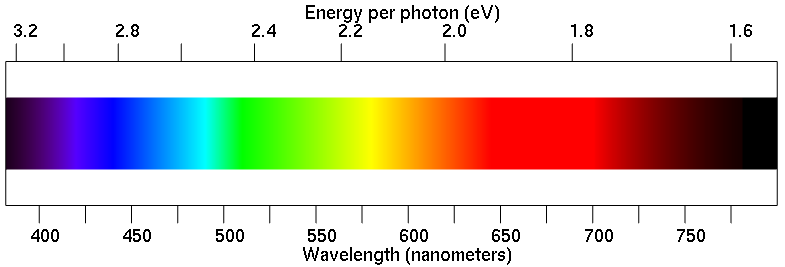
\includegraphics[width=\textwidth]{spectrum2.png}
\end{minipage}

\begin{minipage}{0.33\textwidth}
	What color \\does this appear?
\end{minipage}
\begin{minipage}{0.33\textwidth}
	What element is it?
\end{minipage}
\begin{minipage}{0.33\textwidth}
	What spectral lines did\\
	you use to identify it?
\end{minipage}

\vspace{1.2in}

\begin{minipage}{0.1\textwidth}
	\begin{center}
		\Large Source \\ E
	\end{center}
\end{minipage}
\begin{minipage}{0.7\textwidth}
	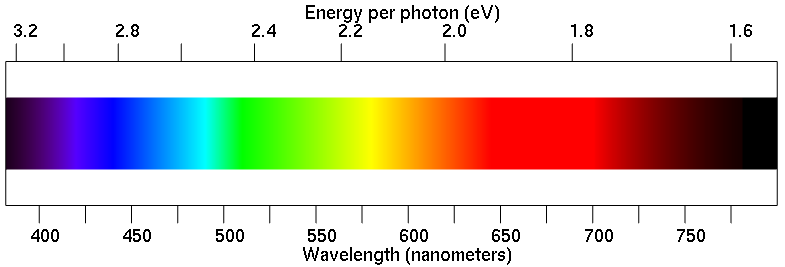
\includegraphics[width=\textwidth]{spectrum2.png}
\end{minipage}

\begin{minipage}{0.33\textwidth}
	What color \\does this appear?
\end{minipage}
\begin{minipage}{0.33\textwidth}
	What element is it?
\end{minipage}
\begin{minipage}{0.33\textwidth}
	What spectral lines did\\
	you use to identify it?
\end{minipage}

\vspace{1.0in}

\begin{minipage}{0.1\textwidth}
	\begin{center}
		\Large Source \\ F
	\end{center}
\end{minipage}
\begin{minipage}{0.7\textwidth}
	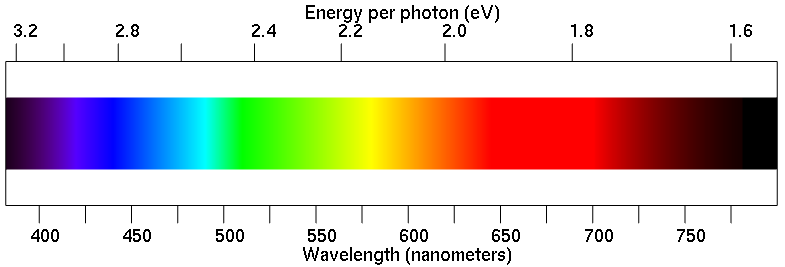
\includegraphics[width=\textwidth]{spectrum2.png}
\end{minipage}

\begin{minipage}{0.33\textwidth}
	What color \\does this appear?
\end{minipage}
\begin{minipage}{0.33\textwidth}
	What element is it?
\end{minipage}
\begin{minipage}{0.33\textwidth}
	What spectral lines did\\
	you use to identify it?
\end{minipage}

\vspace{1.0in}

\newpage
\begin{landscape}
	
	\begin{center}
		\Large 
		Predicting the Colors of Hydrogen
	\end{center}
	
	\large 
	In class we learned about {\it atomic energy levels}. In general, the formula for the energy levels of atoms is very complicated (and there are lots and lots of them!)
	
	But hydrogen is simple. Its energy levels follow a pattern:
	
	$$\text{Energy of level n} = 13.6 \times \frac{n^2-1}{n^2} \text{ electron volts (eV)}.$$
	
	We name these levels by writing $n=$ and then a number. So $n=1$ is the lowest, $n=2$ is the next one, and so on.
	
	An ``electron volt'' is just a very small amount of energy useful for talking about atoms. There are $2.6 \times 10^{22}$) eV in a food-Calorie.
	
	The law of conservation of energy tells us how atoms changing energy levels will relate to light:
	
	
	\begin{itemize}
		\item If an atom jumps to a {\bf higher} energy level, it needs to {\bf take} energy from something, and so it must  {\bf absorb} a photon with energy equal to the difference
		\item If an atom jumps to a {\bf lower} energy level, it needs to {\bf give} energy to something, and so it must {\bf produce} a photon with energy equal to the difference
	\end{itemize}
	
	Remember that each color goes with photons of a specific energy. So this means:
	
	{\bf If you know the energy levels of an atom, you can figure out its emission spectrum by calculating all 
		the different differences between them!}
	
	On the next page, I've calculated the energies for the first five energy levels of hydrogen. (You won't need to use the formula above; I've done it for you.)
	
	\newpage
	Below, I've given you the amounts for the first five energy levels of hydrogen. You can fill out the table and predict the colors that hydrogen can emit and absorb. Label those colors on the spectrum with your pencil... then find the hydrogen lamp in this room
	and see if it matches!
	
	\bigskip
	
	\large
	\begin{tabular}{|c|c|c|c|c|c|c|c|c|}
		\hline
		Higher energy level (to the right) & \multicolumn{2}{c|}{\textbf{\begin{tabular}[c]{@{}c@{}}n=5\\ 13.06 eV\end{tabular}}} & \multicolumn{2}{c|}{\textbf{\begin{tabular}[c]{@{}c@{}}n=4\\ 12.75 eV\end{tabular}}} & \multicolumn{2}{c|}{\textbf{\begin{tabular}[c]{@{}c@{}}n=3\\ 12.09 eV\end{tabular}}} & \multicolumn{2}{c|}{\textbf{\begin{tabular}[c]{@{}c@{}}n=2\\ 10.20 eV\end{tabular}}} \\ \hline
		Lower energy level (below)         & Energy                                    & Color                                   & Energy                                   & Color                                    & Energy                                   & Color                                    & Energy                                   & Color                                    \\ \hline
		\textbf{n=1, 0 eV}                 & 13.06-0=13.06                               & Ultraviolet                             &                                          &                                          &                                          &                                          &                                          &                                          \\ \hline
		\textbf{n=2, 10.20 eV}              &                             &                                   &                                          &                                          &                                          &                                          & -                        & -                        \\ \hline
		\textbf{n=3, 12.09 eV}              &                              &                                 &                                          &                                          & -                        & -                        & -                        & -                        \\ \hline
		\textbf{n=4, 12.75 eV}              & 13.06-12.75=0.31                             & Infrared                                & -                        & -                        & -                        & -                        & -                        & -                        \\ \hline
	\end{tabular}
	
	\bigskip
	
	\begin{minipage}{1in}
		\large
		$E > 3.2$ eV\\
		Ultraviolet
	\end{minipage}
	\begin{minipage}{8in}
		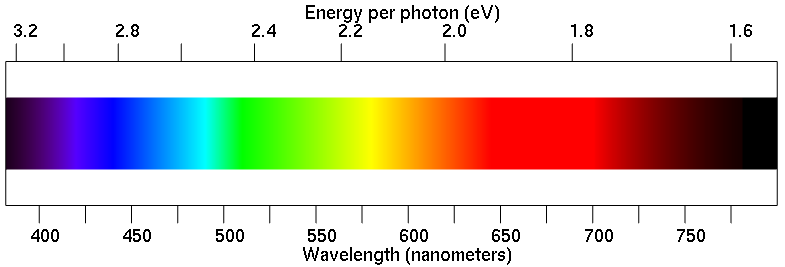
\includegraphics[width=\textwidth]{spectrum2.png}
	\end{minipage}
	\begin{minipage}{1in}
		$E < 1.6$ eV\\
		Infrared
	\end{minipage}
	
	
	\vspace{1in}
	
	Now you can go find the hydrogen lamp in the room and label it on your previous pages.
	
\end{landscape}

\section{ What's in the Room Lights?}

The lights in Holden Observatory work on the same principle as the gas discharge tubes, so by looking at their
spectrum, you should be able to deduce what element is in them.

However, there are a few things that might confound the spectrum that you're seeing:

\begin{itemize}


\item Colored glass might reduce or eliminate certain spectral lines. For instance, red glass allows only red light to pass through it, and blocks other colors. Another sort of tinted glass might block blue and allow other colors to pass. However, remember that {\it colored glass can never create new lines that aren't part of the element's spectrum}.

\item The gas in the room lights also emits a lot of ultraviolet light in addition to the visible colors. This light is useless to our eyes. However, the tubes are coated in {\it phosphors}, which have a molecular structure that causes them to absorb ultraviolet and re-emit {\it broad} spectrum light in the visible. Remember that these phosphors don't create new {\it lines}; they only add broad bands of color on top of the lines from the actual element in the tubes.

\end{itemize}

Looking back at your measurements from the discharge tubes, determine what gas is in the lights in the room. 
\bigskip

\section{ What's In The Sign?}

The ``Experience Physics'' sign outside the auditorium has four different colors: pink, white, blue, and red. Now you'll go do some detective work to figure out what they are. Walk over to the Physics Building.

Remember: Some of the tubes use phosphors that generate {\it broad bands} of color in addition to the narrow spectral
lines produced by the gas itself. Don't get distracted by these: look only at the thin lines in the spectrum.

Based on what you
did before, what elements are used in the different tubes?

\begin{minipage}{0.1\textwidth}
	\begin{center}
		``Experi-\\ence''
	\end{center}
\end{minipage}
\begin{minipage}{0.8\textwidth}
	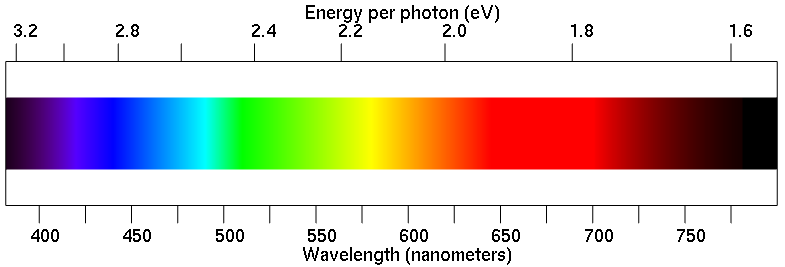
\includegraphics[width=\textwidth]{spectrum2.png}
\end{minipage}


\begin{minipage}{0.33\textwidth}
	What color \\does this appear?
\end{minipage}
\begin{minipage}{0.33\textwidth}
	What element is it?
\end{minipage}
\begin{minipage}{0.33\textwidth}
	What spectral lines did\\
	you use to identify it?
\end{minipage}

\vspace{1.2in}



\begin{minipage}{0.1\textwidth}
	\begin{center}
		\large ``Physics''
	\end{center}
\end{minipage}
\begin{minipage}{0.7\textwidth}
	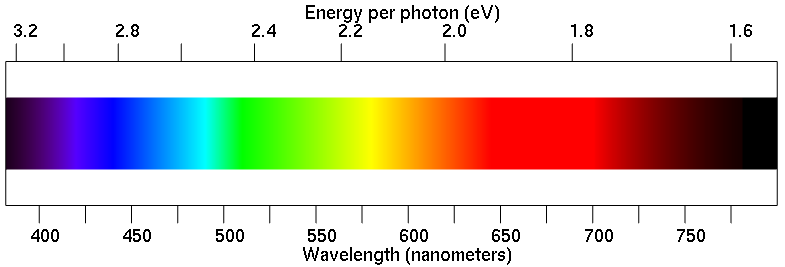
\includegraphics[width=\textwidth]{spectrum2.png}
\end{minipage}

\begin{minipage}{0.33\textwidth}
	What color \\does this appear?
\end{minipage}
\begin{minipage}{0.33\textwidth}
	What element is it?
\end{minipage}
\begin{minipage}{0.33\textwidth}
	What spectral lines did\\
	you use to identify it?
\end{minipage}

\vspace{1.2in}
\hrule



\begin{minipage}{0.1\textwidth}
	\begin{center}
		\large Yellow
	\end{center}
\end{minipage}
\begin{minipage}{0.7\textwidth}
	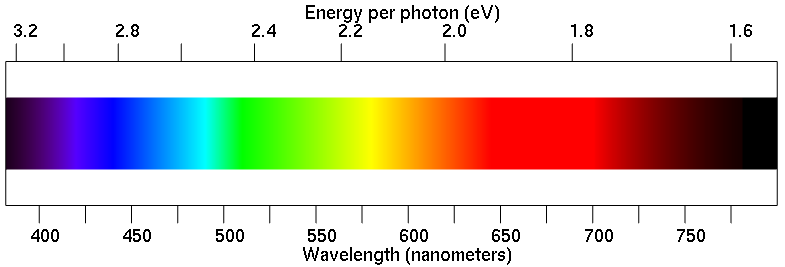
\includegraphics[width=\textwidth]{spectrum2.png}
\end{minipage}

\begin{minipage}{0.33\textwidth}
	What color \\does this appear?
\end{minipage}
\begin{minipage}{0.33\textwidth}
	What element is it?
\end{minipage}
\begin{minipage}{0.33\textwidth}
	What spectral lines did\\
	you use to identify it?
\end{minipage}

\vspace{1.2in}
\hrule
\begin{minipage}{0.1\textwidth}
	\begin{center}
		\large White
	\end{center}
\end{minipage}
\begin{minipage}{0.7\textwidth}
	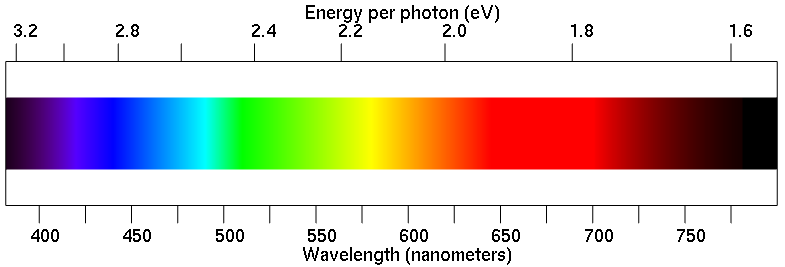
\includegraphics[width=\textwidth]{spectrum2.png}
\end{minipage}


\begin{minipage}{0.33\textwidth}
	What color \\does this appear?
\end{minipage}
\begin{minipage}{0.33\textwidth}
	What element is it?
\end{minipage}
\begin{minipage}{0.33\textwidth}
	What spectral lines did\\
	you use to identify it?
\end{minipage}

\vspace{1.2in}

\newpage

\section{The solar spectrum}

Here is that high-resolution image of the solar spectrum from class. It is broken into stripes; each one is 6 nm
wide. The scale to the right of the image shows the wavelength (in nm) and the photon energy (in eV).
\begin{center}
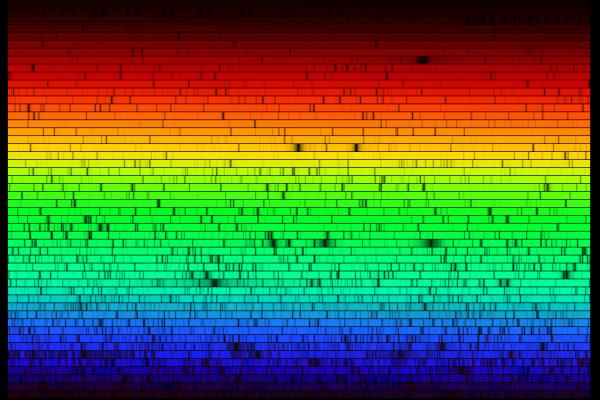
\includegraphics[width=1.0\textwidth]{solarspectrum.jpg}
\end{center}

Try to match some of the lines you measured (or calculated, for hydrogen) with the features shown above
in the Sun's spectrum. Notice that some elements like mercury aren't very common in the Sun.

Try to find:

\begin{itemize}
\item The absorption line corresponding to the $n=3 \rightarrow n=2$ transition in hydrogen
\item The absorption line corresponding to the $n=4 \rightarrow n=2$ transition in hydrogen. (Note that because of things being rounded differently, you may find it closer to 2.54 eV here.)
\item The yellow line that you saw in the sodium lamp and in the reference. Notice that this is really
{\it two} lines, close together; you can see this in the detailed solar spectrum.)
\end{itemize}

Circle these features as you find them.

If you have a nighttime lab, go look at the street lights in the parking lot next to Holden. Figure out what element is in them!


\begin{center}
	
	\begin{landscape}
		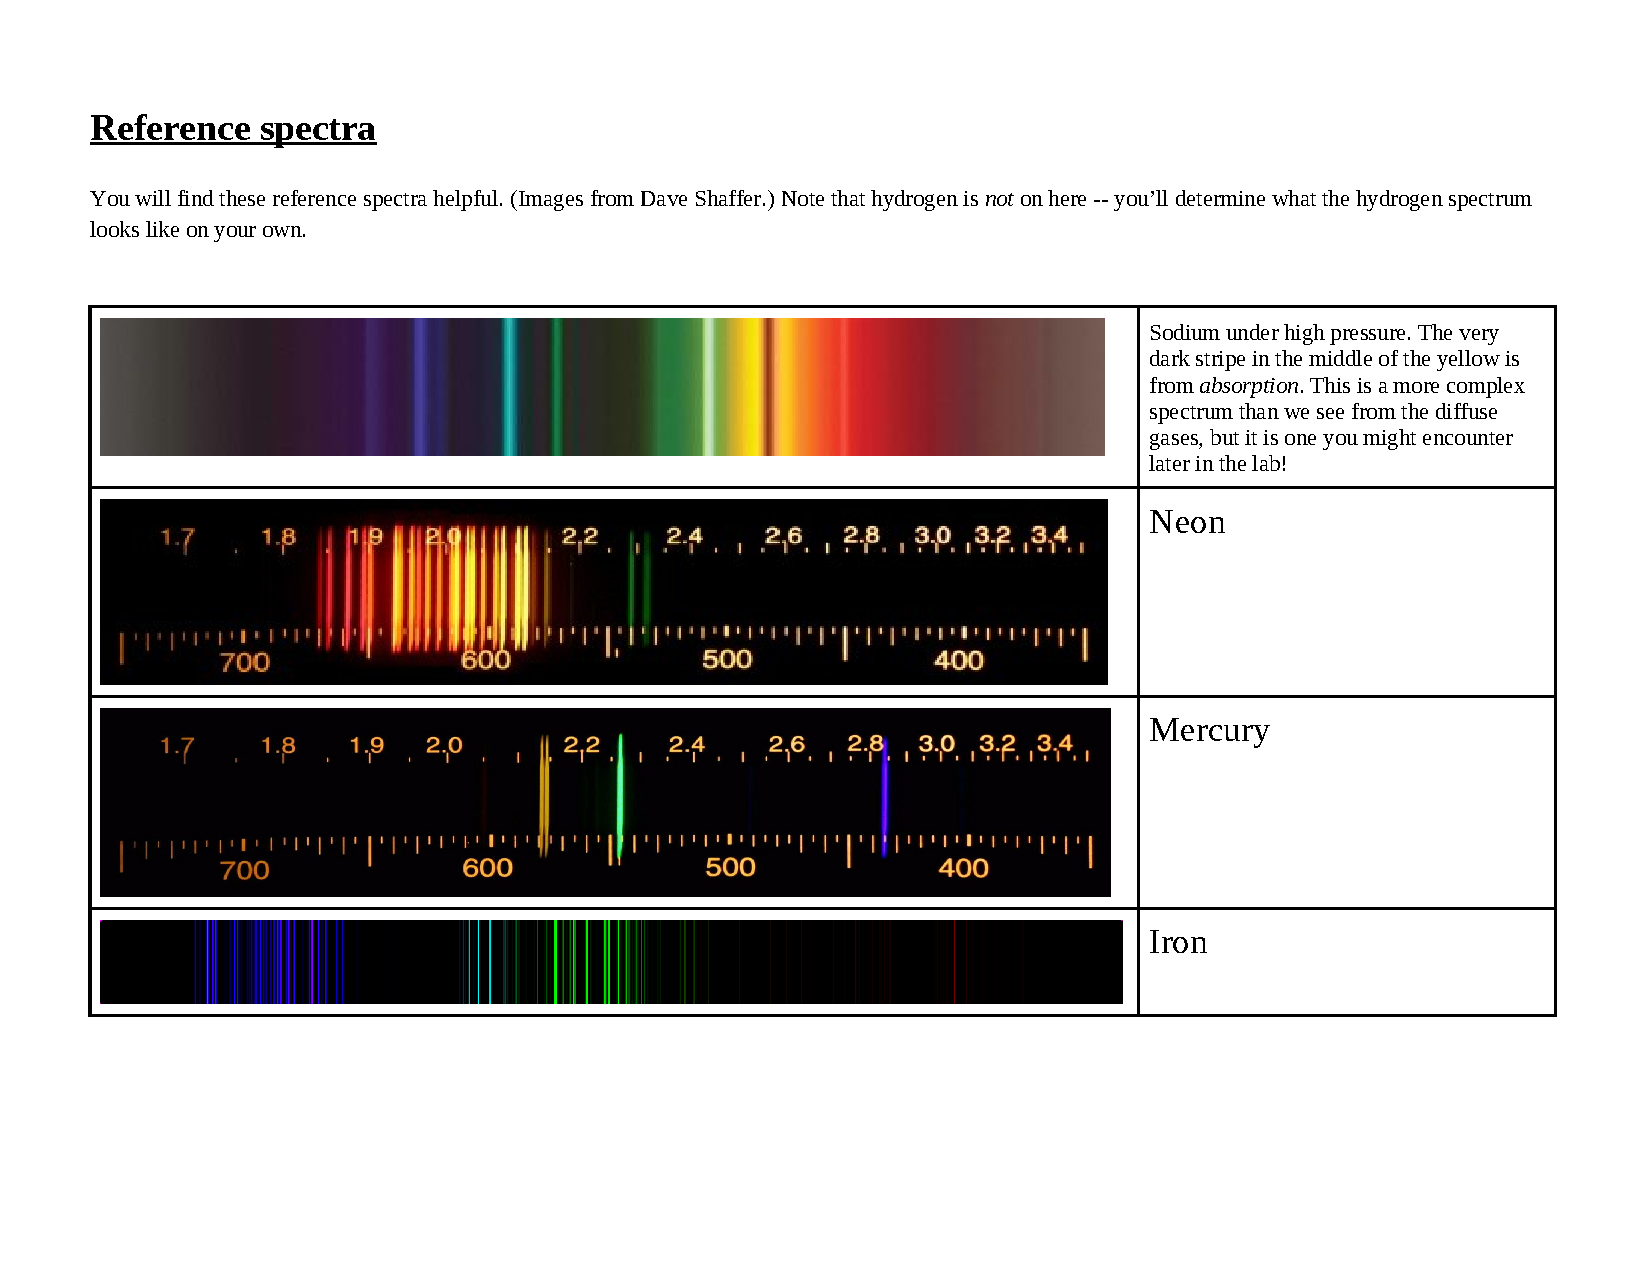
\includepdf[pages=-, angle=-90,width=8in]{reference-spectra.pdf}		
	\end{landscape}
	
\end{center}
\newpage

\end{document}
